\begin{frame}{Sampling $z'$ from vMF}
  \begin{algorithm}[H]
    \caption{Overview of the sampling method from $\mathcal{S}(\mu, \kappa)$}\label{alg:overviewsampling}
    \begin{algorithmic}[1]
      \STATE Sample $z \sim q(z| e_1, \kappa)$ where $e_1 = (1, 0, \dots, 0)$
      \STATE Compute Householder reflection $U(\mu)$ so that $U(\mu) e_1 = \mu$
      \RETURN $z' = U(\mu) z$
    \end{algorithmic}
    \end{algorithm}
  \end{frame}

  \begin{frame}{Sampling $z$ from vMF}
    \begin{algorithm}[H]
      \caption{Overview of the sampling method from $\mathcal{S}(\mu, \kappa)$}\label{alg:overviewsampling2}
      \begin{algorithmic}[1]
        \STATE Sample $z \sim q(z| e_1, \kappa)$ where $e_1 = (1, 0, \dots, 0)$
        \textcolor{red}{
          \STATE Sample $w \in \mathbb{R} \sim g(w |\kappa)$ by acceptance rejection sampling
          \STATE Sample $v \in \mathbb{R}^{d-1} \sim \mathcal{U}(S^{d-2})$ (uniform on the hypersphere $S^{d-2}$)
          \STATE $z \gets (w, \sqrt{1 - w^2}v^T)^T$
        }
        \textcolor{gray}{
        \STATE Compute Householder reflection $U(\mu)$ so that $U(\mu) e_1 = \mu$
        \RETURN $z' = U(\mu) z \sim q(z' | \mu, \kappa)$}
      \end{algorithmic}
      \end{algorithm}
    \end{frame}
  
\begin{frame}{Sampling $w$ from $g(w|\kappa, \theta)$}
  \centering
  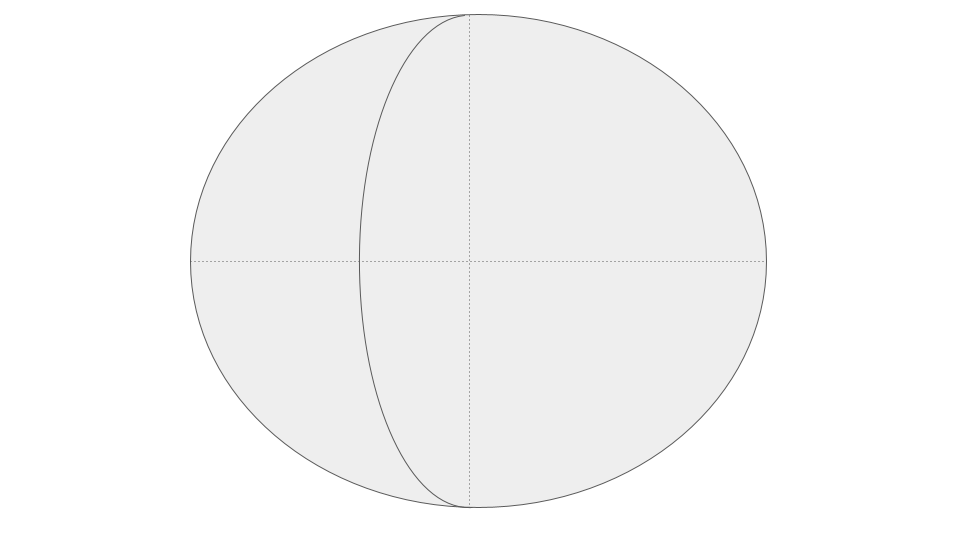
\includegraphics[width=\textwidth]{figures/illustration_sampling_1.png}
  $S^{2}$ : unit sphere in $\mathbb{R}^{3}$
\end{frame}

\begin{frame}{Sampling $w$ from $g(w|\kappa, \theta)$}
  \centering
  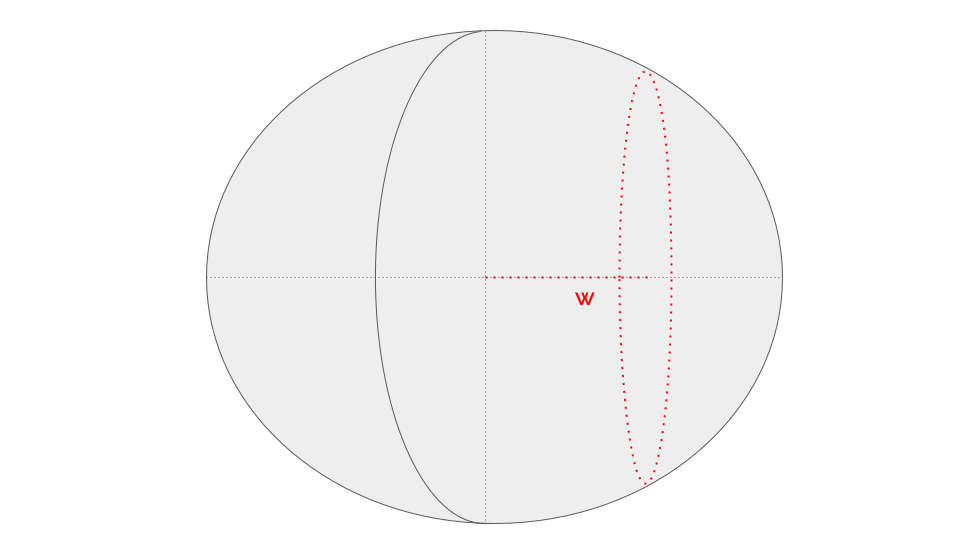
\includegraphics[width=\textwidth]{figures/illustration_sampling_2.png}  
  Sample $w \in \mathbb{R} \sim g(w |\kappa, d)$ by acceptance rejection sampling
\end{frame}

\begin{frame}{Sampling $w$ from $g(w|\kappa)$}
  \begin{itemize}
    \item Case $d=3$
    \item Case $d>3$
  \end{itemize}
\end{frame}

\begin{frame}{Sampling $w$ from $g(w|\kappa)$}
  \centering
  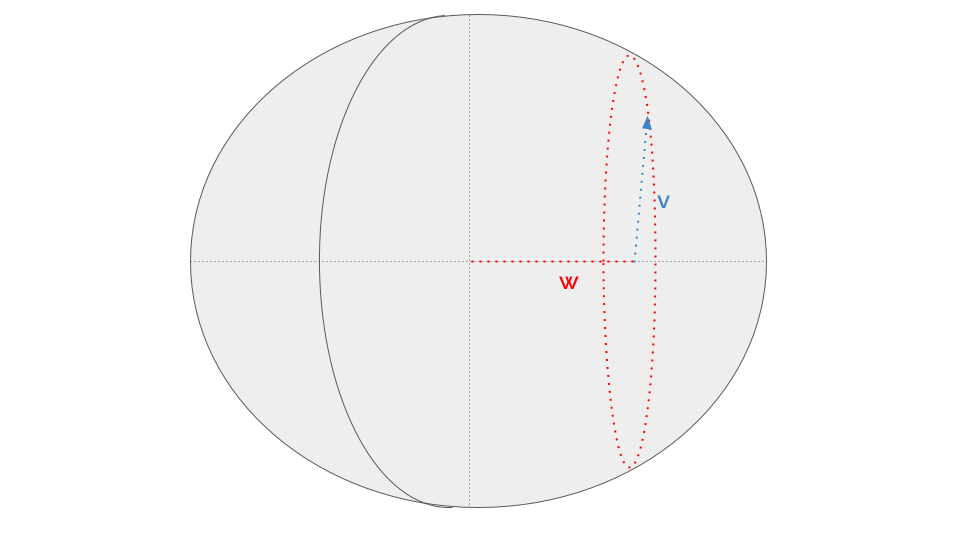
\includegraphics[width=\textwidth]{figures/illustration_sampling_3.png}
  \textcolor{blue}{Sample $v \in \mathbb{R}^{d-1} \sim \mathcal{U}(S^{d-2})$}
\end{frame}

\begin{frame}{Sampling $z$ from $q(z|e_1, \kappa)$}
  \centering
  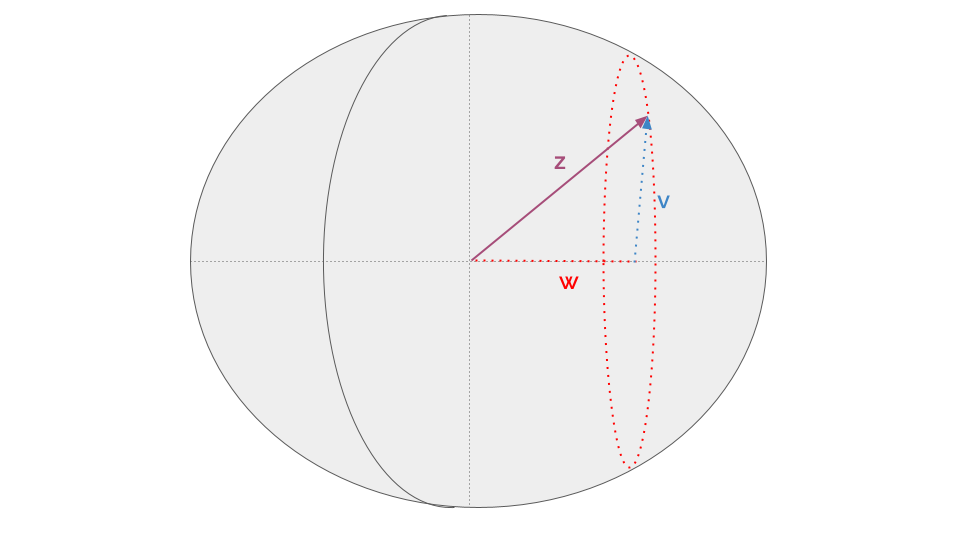
\includegraphics[width=\textwidth]{figures/illustration_sampling_4.png}
  \textcolor{magenta}{$z = (w, \sqrt{1 - w^2}v^T)^T$}
\end{frame}

\begin{frame}{Transform $z$}
  \begin{algorithm}[H]
    \caption{Overview of the sampling method from $\mathcal{S}(\mu, \kappa)$}\label{alg:overviewsampling3}
    \begin{algorithmic}[1]
      \STATE \textcolor{gray}{ Sample $z \sim q(z| e_1, \kappa)$ where $e_1 = (1, 0, \dots, 0)$ }
      \STATE Compute Householder reflection $U(\mu)$ so that $U(\mu) e_1 = \mu$
      \textcolor{red}{
      \STATE $u \gets Normalize(e_1 - \mu)$ 
      \STATE $U \gets I - 2uu^T$}
      \RETURN $z' = U(\mu) z$
    \end{algorithmic}
    \end{algorithm}
\end{frame}